\documentclass[11pt]{article}

\usepackage{amsmath,amssymb,amsthm}
\usepackage{stmaryrd}
\usepackage{mathtools}
\usepackage{tikz-cd}
\usepackage{hyperref}
\usepackage[margin=1in]{geometry}

% LuaLaTeX Unicode support. fontspec lets us choose a Unicode-capable
% monospace font so that Agda identifiers inside \texttt{...} (which
% contain α, σ, ⊗, ⇒, ᵉ, ᴹ, ᵀ, ≈, ℰ, …) render correctly. Math mode
% still uses LaTeX commands (\alpha, \otimes, …) routed through
% Latin Modern Math, so unicode-math is not needed (and conflicts
% with stmaryrd's symbol redefinitions). The one glyph DejaVu Sans
% Mono lacks (ℰ = U+2130 Script capital E) is mapped to math mode.
\usepackage{fontspec}
\setmonofont{DejaVuSansMono}[Scale=MatchLowercase]
\usepackage{newunicodechar}
\newunicodechar{ℰ}{\ensuremath{\mathcal{E}}}

\newtheorem{theorem}{Theorem}
\newtheorem{lemma}[theorem]{Lemma}
\newtheorem{proposition}[theorem]{Proposition}
\newtheorem{construction}[theorem]{Construction}
\newtheorem*{remark}{Remark}

\newcommand{\Set}{\mathbf{Set}}
\newcommand{\Cat}{\mathbf{Cat}}
\newcommand{\SFunM}{\mathbf{SFunM}}
\newcommand{\op}{^{\mathrm{op}}}
\newcommand{\id}{\mathrm{id}}
\newcommand{\Hom}{\mathrm{Hom}}
\newcommand{\Obj}{\mathrm{Obj}}
\newcommand{\bind}{\mathbin{>\!\!\!>\!\!=}}
\newcommand{\ret}{\mathrm{return}}
\newcommand{\stepRel}{\mathrm{stepRel}}
\newcommand{\Channel}{\mathbf{Channel}}
\newcommand{\Machine}{\mathbf{Machine}}
\newcommand{\Maybe}{\mathrm{Maybe}}

\title{From stateful monadic functions to a category of machines}
\author{Categorical Crypto}
\date{}

\begin{document}
\maketitle

\begin{abstract}
We construct the category $\Machine$ whose objects are bidirectional
typed channels and whose morphisms are stateful processes
(``machines'') by stacking five well-known categorical constructions
on top of a commutative, extensional, iterative monad $M$.  The end
result equips the relational process calculus of \texttt{Machine.Core}
with the categorical structure of a traced compact-closed
graded-Kleisli category, transporting categorical laws (associativity,
identity, congruence of composition) along a bijection of hom-sets
rather than proving them by per-axiom bisimulation.
\end{abstract}

\section{Setup}
\label{sec:setup}

We work in $\mathbf{Type}$, the category of types and (computable)
functions. Fix a monad $(M, \ret, \bind)$ on $\mathbf{Type}$ together
with

\begin{itemize}
  \item \emph{extensionality} of bind: substitution under bind
        respects pointwise equality of continuations (see
        Appendix~\ref{sec:background});
  \item \emph{commutativity}: independent binds commute;
  \item an \emph{iteration} operator
        $\mathrm{iter} : (X \to M(X + A)) \to X \to M(A)$ satisfying the
        Bloom--\'Esik axioms~\cite{BloomEsik} (fixpoint, congruence,
        naturality, parameter, codiagonal-$X$, codiagonal-$Y$,
        vanishing-$2$, uniformity).  Codiagonal-$Y$ is the
        symmetric counterpart of codiagonal that starts the
        Bek\v{c}i\'c unfolding on the right summand; vanishing-$2$
        is the nested-iter law identifying $\mathrm{iter}\,fy \bind
        \mathrm{dispatch}$ with $\mathrm{iter}\,(\mathrm{combine}\,fx\,fy)$;
  \item a ``relations-into-$M$'' map (\S\ref{sec:MonadOfRel}) used
        when bridging relational machines to functional homs.
\end{itemize}

Throughout, we write $f \circ g$ for composition in $\mathbf{Type}$ and
$f \mathbin{;}_K g$ for Kleisli composition $f \bind \lambda x. \, g(x)$
in the Kleisli category of $M$.

\section{Construction}

\subsection{Step 1: the category $\SFunM$ of stateful monadic functions}

The Agda record \texttt{SFunM.SFunᵉ} packages a morphism as a hidden
\texttt{State} type with an \texttt{init} value and a step function
\texttt{fun : State × A → M (State × B)}.  See
Appendix~\ref{sec:sfunm} for the categorical background on stateful
monadic functions.

\begin{construction}
The category $\SFunM$ has
\begin{itemize}
  \item objects: types $A$,
  \item morphisms $A \to B$: triples $(S, s_0, f)$ where
        $S$ is a hidden \emph{state} type, $s_0 : S$ an
        \emph{initial state}, and $f : S \times A \to M(S \times B)$.
\end{itemize}
Composition $(T, t_0, g) \circ (S, s_0, f) = (T \times S, (t_0, s_0), g \circ' f)$
where
\[
  (g \circ' f)((t, s), a) = f(s, a) \bind \lambda (s', b).\,
                            g(t, b) \bind \lambda (t', c).\,
                            \ret((t', s'), c).
\]
Identity is $(\{\star\}, \star, (s, a) \mapsto \ret(s, a))$.
\end{construction}

Composition is \texttt{SFunM.\_∘ᵉ\_}; the identity is
\texttt{SFunM.idᵉ}; the category instance is
\texttt{SFunM.SFunᵉ-Category}.  The category laws
(\texttt{assoc-∘ᵉ}, \texttt{identityˡ-∘ᵉ}, \texttt{identityʳ-∘ᵉ},
\texttt{∘ᵉ-resp-≈ᵉ}) reduce to the monad laws plus extensionality of
bind (\texttt{Class.Monad.Ext.ExtensionalMonad}; see
Appendix~\ref{sec:extbind}).

\subsection{Step 2: monoidal structure $(\sqcup, \bot)$ on $\SFunM$}

For category-theory background on (braided / symmetric) monoidal
categories, see Appendices~\ref{sec:monoidal} and~\ref{sec:braided}.

\begin{construction}
For $f : A \to B$ and $g : C \to D$ in $\SFunM$, define
$f \sqcup g : A + C \to B + D$ by
\[
  (f \sqcup g)((s_f, s_g), \mathrm{inj}_1 a) = f(s_f, a) \bind \lambda (s_f', b).\,
                                                \ret((s_f', s_g), \mathrm{inj}_1 b)
\]
and symmetrically on the right summand.  The unit is the empty type
$\bot$.
\end{construction}

The tensor is \texttt{SFunM.Monoidal.\_⊗ᵉ\_}; the symmetric monoidal
instance is \texttt{SFunM.Monoidal.SFunᵉ-monoidal}, extended with
\texttt{Traced.symmetric-ᵉ} for the braiding.  Associator
\texttt{α⇒ᵉ}/\texttt{α⇐ᵉ}, unitors, and braiding \texttt{σᵉ} are all
\texttt{pure-reshape}s of the underlying coproduct on $\mathbf{Type}$;
the pentagon, triangle and hexagon coherences reduce, via the
$\bind$/$\ret$ laws and extensionality, to ordinary coherence in
$(\mathbf{Type}, +, 0)$.

\subsection{Step 3: traced structure on $\SFunM$}

For background on traced monoidal categories see
Appendix~\ref{sec:traced}.

\begin{construction}
For $f : A \sqcup X \to B \sqcup X$ in $\SFunM$, define
\[
  \mathrm{tr}_X(f) : A \to B
\]
by iterating $f$ through the $X$ component: on input $a \in A$ feed
$\mathrm{inj}_1 a$ into $f$; whenever $f$ outputs $\mathrm{inj}_2 x$,
re-feed $\mathrm{inj}_2 x$ until $f$ emits $\mathrm{inj}_1 b$, then
output $b$.  Concretely
\[
  \mathrm{tr}_X(f)(s, a) = \mathrm{iter}\bigl(
      \lambda x.\, f(s, x) \bind \mathrm{tag}\bigr)(\mathrm{inj}_1 a)
\]
where $\mathrm{tag}$ routes $\mathrm{inj}_1 b$ to ``done'' and
$\mathrm{inj}_2 x$ to ``loop''.
\end{construction}

The trace is \texttt{SFunM.Traced.tr}, built on top of two helpers
\texttt{tr-step} (the iter body) and \texttt{tr-cont} (the routing
into loop/done).  The iteration operator \texttt{iter} and its
axioms live in \texttt{Class.Monad.Iterative.IterativeMonad}.

\begin{lemma}\label{lem:traced}
The operator $\mathrm{tr}$ satisfies the Joyal--Street--Verity traced
monoidal axioms:
\begin{itemize}
  \item \emph{vanishing}: $\mathrm{tr}_\bot = \id$ and
        $\mathrm{tr}_{X \sqcup Y} = \mathrm{tr}_X \circ \mathrm{tr}_Y$
        (modulo a coherence isomorphism),
  \item \emph{superposing}:
        $\mathrm{tr}_X(\id_Y \sqcup f) = \id_Y \sqcup \mathrm{tr}_X(f)$,
  \item \emph{yanking}: $\mathrm{tr}_X(\sigma) = \id_X$ where
        $\sigma$ is the braiding.
\end{itemize}
\end{lemma}

In Agda, each axiom is a top-level theorem:
\texttt{Traced.vanishing₁-ᵉ}, \texttt{Traced.vanishing₂-ᵉ},
\texttt{Traced.superposing-ᵉ}, \texttt{Traced.yanking-ᵉ}.  Vanishing-1
(\texttt{vanishing₁-ᵉ}) and yanking (\texttt{yanking-ᵉ}) follow from
\texttt{iter-fix} plus monad laws.  Superposing
(\texttt{superposing-ᵉ}) and the X-direction of vanishing-2 use
\texttt{iter-codiag} and \texttt{iter-conjugate} (Hasegawa
uniformity~\cite{Hasegawa97}).  The Y-direction of vanishing-2 needs
two further axioms beyond the standard Bloom--\'Esik six:
\texttt{iter-codiag-y} (the symmetric Bek\v{c}i\'c unfolding) and
\texttt{iter-vanishing-2} (collapsing nested $\mathrm{iter}$s into a
single $\mathrm{iter}$ on \texttt{combine}).  Both are bundled into
\texttt{IterativeMonad} and used by the bridging lemma
\texttt{iter-equiv-final-y}.

The traced instance is \texttt{Traced.SFunᵉ-traced}, exposing the
\texttt{Traced} record from \texttt{agda-categories}.

\subsection{Step 4: the G-construction (``Int'' / geometry of interaction)}

The Joyal--Street--Verity G-construction (see
Appendix~\ref{sec:gconstr} for the definition and theorem) takes a
traced symmetric monoidal category $\mathcal{C}$ and produces a
compact-closed category $G\mathcal{C}$ whose objects are pairs
$(A^+, A^-) \in \Obj(\mathcal{C})^2$ and whose homs are
$G\mathcal{C}((A^+, A^-), (B^+, B^-)) = \mathcal{C}(A^+ \otimes B^-,\,
A^- \otimes B^+)$.

\paragraph{Applied here.}  Take $\mathcal{C} = \SFunM$ with
$(\otimes, I) = (\sqcup, \bot)$.  Then
\[
  \Hom_{G\SFunM}((A^+, A^-), (B^+, B^-))
  = \Hom_\SFunM(A^+ \sqcup B^-,\, A^- \sqcup B^+),
\]
i.e.\ stateful monadic functions that, given an input on either the
``A-input side'' or the ``B-output side'', emit on either the
``A-output side'' or the ``B-input side''.  This is the exact
typed-channel shape used by \texttt{Channel.Core}.

In Agda the G-construction is parameterised over an arbitrary traced
symmetric monoidal $\mathcal{C}$ in \texttt{Categories.GConstruction};
the instantiation at $\SFunM$ is
\texttt{Machine.Category.SFunᵉ-GConstruction}.

\subsection{Step 5: Maybe-graded Kleisli over $G\SFunM$}

For the definition of a graded monad and its graded Kleisli
category see Appendix~\ref{sec:graded}.

\paragraph{Applied here.}  We grade $G\SFunM$ by the terminal
monoidal category $\mathbf{1}$ (so all subsumption maps collapse
to identities), and pick the \emph{Maybe-augmenting} monad
\[
  T_\star(A^+, A^-) \;:=\; (A^+ \sqcup \top,\; A^-).
\]
Adding a $\top$ alternative to the positive component of a G-object
means that a $\mathrm{Kl}_T$-morphism
$A \to T_\star(B)$ in $G\SFunM$ unfolds to
\[
  \SFunM(A^+ \sqcup B^-,\; A^- \sqcup (B^+ \sqcup \top))
  \;\;\cong\;\;
  \SFunM(A^+ \sqcup B^-,\; \Maybe(A^- \sqcup B^+))
\]
via the canonical iso $\Maybe X \cong X \sqcup \top$ together with
associativity of $\sqcup$.  That right-hand hom-set is exactly the
``$\Maybe$-augmented'' shape used by $\Machine$'s \texttt{stepRel}
(see Step~6): given an input on either side of the channel, the
morphism either emits on either side or stays silent ($\top$).

\paragraph{Unit and Kleisli extension.}
The graded unit at $A$,
$\eta_A : A \to T_\star(A)$, is the G-construction identity (the
braiding $\sigma$) post-composed with the canonical
$\mathrm{inj}_1 : A^+ \to A^+ \sqcup \top$.  The Kleisli extension
$\mathrm{ext} : (A \to T_\star B) \to (T_\star A \to T_\star B)$
pattern-matches on the $A^+ \sqcup \top$-typed input: the new $\top$
case emits ``no output'' on the $B^+ \sqcup \top$ side, while every
other input is forwarded to the underlying morphism.

In Agda these are \texttt{MaybeT₀}, \texttt{MaybeT-return}, and
\texttt{MaybeT-ext} in \texttt{Machine.Category}.  They assemble
into \texttt{SFunᵉ-GradedTriple}, which in turn yields the graded
Kleisli category \texttt{SFunᵉ-GradedKleisli} via
\texttt{Categories.GradedKleisli}.  The four sub-only graded-Kleisli
laws (\texttt{sub-identity}, \texttt{sub-homomorphism},
\texttt{sub-resp-≈}) are proved from G-construction identities; the
five $\mathrm{ext}$-related laws are postulated with concrete proof
sketches inline (Tier-3 roadmap).

\subsection{Step 6: machines and the $\Machine \leftrightarrow \mathrm{Hom}$ bijection}

\subsubsection{Channels}

A \emph{channel} $A \in \Channel$ is a pair of types
$(\mathrm{in}_A, \mathrm{out}_A)$ encoding ``messages flowing in''
and ``messages flowing out''.  In Agda this is the record
\texttt{Channel.Core.Channel}; the transpose
$A^T = (\mathrm{out}_A, \mathrm{in}_A)$ is \texttt{\_ᵀ}, the
component-wise coproduct tensor is \texttt{\_⊗₀\_}.

There is an evident isomorphism
\[
  \Channel \xrightarrow{\cong} \Obj(G\SFunM),
  \qquad
  A \mapsto (\mathrm{in}_A, \mathrm{out}_A).
\]

\subsubsection{Machines}

A \emph{machine} $M : A \to B$ in $\Machine$ is a triple
$(S, \stepRel)$ with $S$ a hidden \emph{state} type and
\[
  \stepRel : S \times \mathrm{in}_{A \otimes B^T} \times
             \Maybe(\mathrm{out}_{A \otimes B^T}) \times S \to \Set,
\]
i.e.\ a four-place \emph{relation} parameterised by (current state,
input message, optional output message, next state).  In Agda this
is the record \texttt{Machine.Core.Machine}, with fields
\texttt{State}, \texttt{init}, and \texttt{stepRel}.

Two structural features distinguish this from a $G\SFunM$ hom:
\begin{enumerate}
  \item[(R)] \emph{Relations vs. functions}.  $\stepRel$ is set-valued
       (a relation); a $G\SFunM$ hom is function-valued (into $M$).
  \item[(O)] \emph{Optional output}.  The $\Maybe$ wraps the output
       message; a $G\SFunM$ hom always emits.
\end{enumerate}

\subsubsection{The bridge: $\mathrm{MonadOfRel}$}\label{sec:MonadOfRel}

To turn an arbitrary relation into an $M$-value, we require an
additional structural assumption on $M$:
\[
  \mathrm{ofrel} : (A \to \Set) \to MA, \qquad
  \mathrm{member} : A \to MA \to \Set,
\]
with
\begin{itemize}
  \item $P(a) \iff \mathrm{member}(a, \mathrm{ofrel}(P))$,
  \item $m = \mathrm{ofrel}(\lambda a.\, \mathrm{member}(a, m))$ (extensionality).
\end{itemize}
The canonical instance is $M = \Set^{(-)}$ (the power-set / predicate
monad), where $\mathrm{ofrel} = \id$ and $\mathrm{member}(a, P) = P(a)$.
This data lives in \texttt{Class.Monad.OfRel}.

\subsubsection{The Maybe-augmented hom-set $\mathrm{MaybeHom}$}

To absorb (O) we introduce
\[
  \mathrm{MaybeHom}(A, B) = \bigl\{(S, f) : f : S \times \mathrm{in}_{A \otimes B^T}
                                \to M(S \times \Maybe(\mathrm{out}_{A \otimes B^T}))\bigr\},
\]
i.e.\ a stateful monadic function whose output is wrapped in
$\Maybe$.  This is the categorical analogue of \texttt{Machine.stepRel}
modulo the relation/function bridge.

\paragraph{$\mathrm{MaybeHom}$ as a graded-Kleisli hom-set.}
Up to the canonical iso $\Maybe X \cong X \sqcup \top$ and
$\sqcup$-associativity, $\mathrm{MaybeHom}(A, B)$ is exactly the
hom-set of the Maybe-graded Kleisli category $\mathrm{Kl}_T(G\SFunM)$
from Step~5:
\[
  \mathrm{MaybeHom}(A, B) \;\;\cong\;\;
  \mathrm{Kl}_T(G\SFunM)\bigl((\mathrm{in}_A, \mathrm{out}_A),
                              (\mathrm{in}_B, \mathrm{out}_B)\bigr)
  \;=\; G\SFunM\bigl(A,\, T_\star(B)\bigr).
\]
In Agda the principled version is \texttt{MaybeHom-Kl}, and the iso
is \texttt{MaybeHom→Kl} / \texttt{Kl→MaybeHom}.  The two differ only
in (i) an \texttt{init} field absent from \texttt{MaybeHom} (since
\texttt{Machine} is similarly init-less, and the bijection of Step~6
preserves that), and (ii) the $\Maybe$ vs.\ $\sqcup \top$ shape of
the output.  Under this iso, the four $\mathrm{MaybeHom}$ category
laws are the bijection image of the corresponding
$\mathrm{Kl}_T(G\SFunM)$ laws, which themselves transport from the
Maybe-graded triple's ten Kleisli laws.

\begin{construction}[Bijection]
Define
\begin{align*}
  \mathrm{Machine} \to \mathrm{Hom} &:\qquad
    (S, R) \mapsto (S,\, \lambda(s, i).\, \mathrm{ofrel}(\lambda(s', o).\, R(s, i, o, s'))),\\
  \mathrm{Hom} \to \mathrm{Machine} &:\qquad
    (S, f) \mapsto (S,\, \lambda(s, i, o, s').\, \mathrm{member}((s', o), f(s, i))).
\end{align*}
\end{construction}

\begin{lemma}[Round-trip]
The two arrows are inverse up to:
\begin{itemize}
  \item logical equivalence of $\stepRel$ pointwise (\emph{Machine}-side
        round-trip), and
  \item propositional equality of $M$-values pointwise
        (\emph{MaybeHom}-side round-trip).
\end{itemize}
Both follow from the two $\mathrm{MonadOfRel}$ laws above.
\end{lemma}

\subsection{Step 7: the category $\Machine$}

We finally bundle Channels and Machines as a category.

\begin{construction}
Define
\begin{itemize}
  \item objects: $\Obj(\Machine) = \Channel$;
  \item morphisms: $\Hom_\Machine(A, B) = \Machine(A, B)$;
  \item identity: the obvious stateless ``always-forward'' machine;
  \item composition $M_2 \circ M_1$: tensor the two machines and trace
        out the shared channel (this is the relational analogue of
        $G\SFunM$ composition);
  \item equivalence $\sim_\mathcal{E}$: \emph{perfect indistinguishability
        under environments}, $M_1 \sim_\mathcal{E} M_2$ iff for every
        environment $E : B \to \mathcal{E}$ we have
        $E \circ M_1 = E \circ M_2$ as machines (using whatever
        ambient notion of machine equality).
\end{itemize}
\end{construction}

In Agda the identity is \texttt{Machine.Core.idᴹ}, the tensor product
of machines is \texttt{Machine.Core.\_⊗₁\_}, the trace is
\texttt{Machine.Core.tr} (built from the inductive \texttt{TraceRel}),
composition is \texttt{Machine.Core.\_∘\_}, and the environment-based
equivalence is \texttt{Machine.Core.\_≈ℰ\_}.  The category instance
on $\Machine$ is assembled in \texttt{Machine.Category}.

\begin{theorem}[Categorical laws via transport]
The triple $(\Channel, \Machine, \sim_\mathcal{E})$ satisfies the
category axioms (associativity, left/right identity, congruence of
composition).
\end{theorem}

\begin{proof}[Proof sketch]
$\sim_\mathcal{E}$ is an equivalence because $=$ is.  The other three
laws transport along the bijection of \S~6: any equation
$f \sim_\mathcal{E} g$ for $\Machine$ unfolds, via
$\mathrm{Machine} \to \mathrm{Hom}$, to the corresponding equation in
$\mathrm{MaybeHom}$.  Modulo functoriality of the bijection (which is
immediate from the bijection-induced composition on $\mathrm{MaybeHom}$),
the law in $\mathrm{MaybeHom}$ pulls back to the desired law in
$\Machine$.

The $\mathrm{MaybeHom}$ laws themselves are the categorical residue of
the construction --- they hold whenever
\begin{itemize}
  \item the $G\SFunM$ category laws hold (Step 4),
  \item $\mathrm{MaybeHom}$ composition is the Kleisli composition over
        the appropriate Maybe-graded monad on $G\SFunM$ (a
        substitution of Step 5's graded triple).
\end{itemize}
With the trivial identity graded triple used here, the
$\mathrm{MaybeHom}$ laws reduce to the $G\SFunM$ laws plus a
$\Maybe$-bookkeeping; with a richer triple the
$\Maybe$-augmentation lives inside the categorical machinery itself.
\end{proof}

\section{The whole picture}

\[
\begin{tikzcd}[column sep=large]
  \mathbf{Type} \arrow[r] &
  \SFunM \arrow[r] &
  (\SFunM, \sqcup, \bot) \arrow[r] &
  \text{traced } \SFunM \arrow[d] \\
  \Machine &
  \mathrm{MaybeHom} \arrow[l, "\cong"] &
  \mathrm{Kl}_T(G\SFunM) \arrow[l] &
  G\SFunM \arrow[l]
\end{tikzcd}
\]

\noindent
The horizontal arrows are well-known constructions on a category;
each step is functorial and preserves the structure used by the
next.  In Agda each is a named module:
\begin{itemize}
  \item Kleisli of $M$ over $\mathbf{Type}$: implicit in the use of
        \texttt{Monad} from \texttt{Class.Monad}.
  \item equipping with the coproduct tensor:
        \texttt{SFunM.Monoidal.SFunᵉ-monoidal} (Step 2);
  \item taking the JSV trace: \texttt{SFunM.Traced.SFunᵉ-traced}
        (Step 3);
  \item the $G$-construction: abstract in
        \texttt{Categories.GConstruction}, applied at $\SFunM$ in
        \texttt{Machine.Category.SFunᵉ-GConstruction} (Step 4);
  \item the Maybe-graded Kleisli (trivial $\mathbf{1}$ grading,
        non-trivial $T_\star(A^+, A^-) = (A^+ \sqcup \top, A^-)$):
        \texttt{Categories.GradedKleisli} applied via
        \texttt{Machine.Category.SFunᵉ-GradedKleisli} with the
        Maybe-graded triple \texttt{SFunᵉ-GradedTriple} (Step 5).
\end{itemize}
The final bijection $\mathrm{MaybeHom} \cong \Machine$ uses the
\texttt{Class.Monad.OfRel} bridge to absorb the
relation-vs-function distinction.

\section{Outstanding theoretical content not yet captured constructively}

The following items are mathematically routine but, at present,
postulated in the Agda development:
\begin{itemize}
  \item \emph{Trace naturality} (\S\ref{lem:traced}, $\mathrm{tr}$-resp,
        left/right naturality, Fubini) for $\SFunM$.  Derivable from
        the basic vanishing/superposing/yanking axioms via
        Hasegawa's setoid-level proofs.
  \item $G\SFunM$'s \emph{identity laws} and \emph{associativity
        coherence}.  These are standard for any traced symmetric
        monoidal category but require careful manipulation of
        $\alpha$, $\sigma$, $\gamma$.
  \item Graded Kleisli's category laws (assoc/identity).  Standard
        for any graded monad.
  \item The Machine-extensionality form of the round-trip
        (\emph{propositional} Machine equality, vs.\ stepRel-level
        logical equivalence).
  \item The five $\mathrm{ext}$-related laws of the Maybe-graded
        triple (\texttt{ext-identityˡ}, \texttt{ext-identityʳ},
        \texttt{ext-assoc}, \texttt{ext-resp-≈},
        \texttt{sub-commute}).  These are equations in
        $\SFunM$-$G$-construction's hom-equivalence under list-trace
        evaluation; the file ships Tier-3 proof-sketch comments at
        each postulate.  Once discharged, the four
        $\mathrm{MaybeHom}$ category laws follow by transport through
        the $\mathrm{MaybeHom} \cong \mathrm{MaybeHom\text{-}Kl}$
        iso of Step~6 — modulo also (i) the four upstream holes in
        \texttt{Categories.GradedKleisli}, and (ii) showing the iso
        is functorial.
\end{itemize}

None of these obstructions affect the mathematical claim that
$\Machine$ is a category; they are loose ends in the formal Agda
artefact, listed here for transparency.

\appendix

\section{Categorical background}
\label{sec:background}

This appendix recalls the categorical apparatus used throughout the
main body.  Readers familiar with monads and Kleisli categories can
skim or skip it entirely; readers seeing this material for the first
time may prefer to read the appendix before the main body.

\subsection{Categories and hom-sets}
\label{sec:hom-sets}

A \emph{category} $\mathcal{C}$ consists of
\begin{itemize}
  \item a collection $\Obj(\mathcal{C})$ of \emph{objects};
  \item for each pair $A, B \in \Obj(\mathcal{C})$, a collection of
        \emph{morphisms} (or \emph{arrows}) $A \to B$;
  \item for each $A \in \Obj(\mathcal{C})$, an \emph{identity}
        morphism $\id_A : A \to A$;
  \item a composition operation that, given $f : A \to B$ and
        $g : B \to C$, produces $g \circ f : A \to C$;
\end{itemize}
subject to associativity ($h \circ (g \circ f) = (h \circ g) \circ f$)
and unit laws ($\id_B \circ f = f = f \circ \id_A$).

The collection of morphisms from $A$ to $B$ in $\mathcal{C}$ is the
\emph{hom-set} (or \emph{hom-object}) of $A$ and $B$.  We write it
either as
\[
  \Hom_\mathcal{C}(A, B) \qquad\text{or}\qquad \mathcal{C}(A, B),
\]
with the shorter notation preferred when the category is unambiguous.
The two notations are used interchangeably throughout this document.
A few notational conventions:
\begin{itemize}
  \item ``$f : A \to B$ in $\mathcal{C}$'' is shorthand for
        $f \in \mathcal{C}(A, B)$.
  \item In a category $\mathcal{C}$ with extra structure (e.g.\ a
        monoidal one), the hom-set $\mathcal{C}(A, B)$ may itself
        live in a richer category, e.g.\ a set with topology
        (\emph{topological enrichment}) or a monoidal-category-valued
        \emph{enrichment}.  In this document all hom-sets are plain
        sets.
  \item The hom-set of a derived category, e.g.\ Kleisli
        $\mathcal{C}_T(A, B) = \mathcal{C}(A, T B)$, is computed from
        the underlying $\mathcal{C}$ together with the construction's
        rule.
\end{itemize}

A \emph{small category} is one whose objects and hom-sets are
genuine (small) sets.  Most categories we discuss --- $\Set$,
$\SFunM$, $G\SFunM$, the various Kleisli categories on top --- are
not small in this strict sense (their objects are types, which form
a proper class), but they are locally small (each hom-set is a set).

\subsection{Functors, natural transformations, adjoints}

We freely use the following concepts.

\paragraph{Functors.}
A \emph{functor} $F : \mathcal{C} \to \mathcal{D}$ assigns an object
$F(A) \in \mathcal{D}$ to each $A \in \mathcal{C}$ and a morphism
$F(f) : F(A) \to F(B)$ to each $f : A \to B$, preserving identity
($F(\id_A) = \id_{F(A)}$) and composition
($F(g \circ f) = F(g) \circ F(f)$).  An \emph{endofunctor} is a
functor $F : \mathcal{C} \to \mathcal{C}$.  A \emph{bifunctor} is a
functor from a product category $\mathcal{C} \times \mathcal{D}$,
e.g.\ the tensor product $\otimes : \mathcal{C} \times \mathcal{C}
\to \mathcal{C}$ of a monoidal category.

\paragraph{Natural transformations.}
Given two functors $F, G : \mathcal{C} \to \mathcal{D}$, a
\emph{natural transformation} $\eta : F \Rightarrow G$ is a family of
morphisms $\{\eta_A : F(A) \to G(A)\}_{A \in \mathcal{C}}$ such that
for every $f : A \to B$ in $\mathcal{C}$ the diagram
\[
\begin{tikzcd}
  F(A) \arrow[r, "\eta_A"] \arrow[d, "F(f)"'] & G(A) \arrow[d, "G(f)"] \\
  F(B) \arrow[r, "\eta_B"']                   & G(B)
\end{tikzcd}
\]
commutes (\emph{naturality square}).  If every $\eta_A$ is an
isomorphism, $\eta$ is a \emph{natural isomorphism},
$\eta : F \xrightarrow{\sim} G$.

Naturality is the categorical formalisation of ``$\eta$ is uniformly
defined and doesn't depend on accidental features of $A$'' --- the
square forces it to commute with any morphism between objects.  This
is the key property that makes monad units/multiplications,
monoidal associators/unitors/braidings, and trace operators
\emph{well-behaved}: they automatically slide past arrows.

\paragraph{Adjoints.}
An \emph{adjunction} between categories $\mathcal{C}$ and
$\mathcal{D}$ is a pair of functors $F : \mathcal{C} \to \mathcal{D}$,
$U : \mathcal{D} \to \mathcal{C}$ together with a natural bijection
\[
  \mathcal{D}\bigl(F(A),\, B\bigr) \;\cong\; \mathcal{C}\bigl(A,\, U(B)\bigr),
\]
written $F \dashv U$.  Equivalently, an adjunction is determined by a
unit $\eta : \id_\mathcal{C} \Rightarrow U F$ and a counit
$\epsilon : F U \Rightarrow \id_\mathcal{D}$ satisfying the
\emph{triangle identities}
$(\epsilon F) \circ (F \eta) = \id_F$ and
$(U \epsilon) \circ (\eta U) = \id_U$.

\paragraph{Why this matters here.}
Every monad $(T, \eta, \mu)$ on $\mathcal{C}$ arises from an
adjunction: the functors $J : \mathcal{C} \to \mathcal{C}_T$
(Kleisli) and $U : \mathcal{C}_T \to \mathcal{C}$ with $U(A) = T A$
form an adjunction $J \dashv U$, and the monad is recovered as
$T = U \circ J$ with unit and multiplication coming from $\eta$ and
$\epsilon$.  Symmetrically for the Eilenberg--Moore category
$\mathcal{C}^T$.  This is the conceptual reason both ``derived
categories'' exist canonically (\S\ref{sec:monads-derived}).

\subsection{Monads on a category}
\label{sec:monads-derived}

A \emph{monad} on a category $\mathcal{C}$ is a triple
$(T, \eta, \mu)$ where
\begin{itemize}
  \item $T : \mathcal{C} \to \mathcal{C}$ is an endofunctor,
  \item $\eta : \id_\mathcal{C} \Rightarrow T$ is a natural
        transformation (the \emph{unit}),
  \item $\mu : T T \Rightarrow T$ is a natural transformation (the
        \emph{multiplication}),
\end{itemize}
subject to two coherence equations:
\begin{itemize}
  \item \emph{Associativity}: $\mu \circ T\mu = \mu \circ \mu T$
        as natural transformations $T^3 \Rightarrow T$.
  \item \emph{Unit}: $\mu \circ T\eta = \id_T = \mu \circ \eta T$.
\end{itemize}
This is exactly a monoid object in the endofunctor category
$[\mathcal{C}, \mathcal{C}]$ with $\circ$ as the monoidal product.

A monad on $\mathcal{C}$ doesn't replace the category --- it sits on
top of one and gives rise to \emph{two} canonical new categories built
from $(\mathcal{C}, T)$:

\paragraph{Eilenberg--Moore $\mathcal{C}^T$.}
The objects are \emph{$T$-algebras}: pairs $(A, \alpha)$ with
$\alpha : T A \to A$ satisfying
$\alpha \circ \eta_A = \id_A$ and
$\alpha \circ T\alpha = \alpha \circ \mu_A$.  Morphisms are algebra
homomorphisms.  This is where one studies \emph{models} of the
algebraic theory encoded by $T$.

\paragraph{Kleisli $\mathcal{C}_T$.}
The same objects as $\mathcal{C}$, but the morphisms are
\emph{Kleisli arrows}:
\[
  \mathcal{C}_T(A, B) := \mathcal{C}(A, T B).
\]
Composition reuses $\mu$:
\[
  g \circ_T f := \mu_C \circ T(g) \circ f
            \qquad (\text{equivalently, } g \bind f).
\]
The unit $\eta_A : A \to T A$ is identity in $\mathcal{C}_T$ at object
$A$.  Kleisli composition is associative and unital exactly because of
the monad axioms.

There is a canonical functor $J : \mathcal{C} \to \mathcal{C}_T$
sending $f : A \to B$ to $\eta_B \circ f : A \to T B$ --- every plain
$\mathcal{C}$-morphism is trivially a $T$-computation.  $J$ is part
of an adjunction $J \dashv U$ with right adjoint $U(A) = T A$;
$\mathcal{C}_T$ is the \emph{initial} solution to this
``free $T$-algebra'' problem, while $\mathcal{C}^T$ is the
\emph{terminal} one (Beck's theorem~\cite{Beck}).

\paragraph{Slogan.}
A category lets you compose plain functions.  A monad lets you
compose functions \emph{that may produce a $T$-effect}, by giving you
the categorical apparatus ($\eta, \mu$) to flatten nested effects
($T T \to T$) and inject pure values ($\id \to T$).

\subsection{The Kleisli-triple presentation}

The monad axioms above use both an endofunctor $T$ and a
multiplication $\mu$.  A \emph{Kleisli triple}~\cite{Manes} is an
equivalent presentation that avoids spelling out the functorial
action on morphisms.  A Kleisli triple on $\mathcal{C}$ is
$(T_0, \eta, (-)^*)$ where
\begin{itemize}
  \item $T_0 : \Obj(\mathcal{C}) \to \Obj(\mathcal{C})$ is an action
        on objects only,
  \item $\eta_A : A \to T_0 A$ is the unit, one per object,
  \item $(-)^* : \mathcal{C}(A, T_0 B) \to \mathcal{C}(T_0 A, T_0 B)$
        is the \emph{Kleisli extension}, lifting a Kleisli arrow
        $f : A \to T_0 B$ to a morphism $f^* : T_0 A \to T_0 B$,
\end{itemize}
subject to three axioms:
\begin{enumerate}
  \item $\eta_A^* = \id_{T_0 A}$
  \item $f^* \circ \eta_A = f$
  \item $(g^* \circ f)^* = g^* \circ f^*$
\end{enumerate}

\begin{theorem}[\cite{Manes}]
The data $(T_0, \eta, (-)^*)$ on $\mathcal{C}$ satisfying axioms~1--3
is in bijection with monads $(T, \eta, \mu)$ on $\mathcal{C}$.  The
functor's morphism action is recovered as $T(f) = (\eta_B \circ f)^*$,
and the multiplication as $\mu_A = \id_{T A}^*$.
\end{theorem}

\paragraph{Connection to \texttt{return} and \texttt{bind}.}
If one writes \texttt{bind} as postfix infix:
\[
  f^*(m) = m \bind f,
\]
then the three Kleisli-triple axioms become the familiar three monad
laws:
\begin{enumerate}
  \item $m \bind \ret = m$ (right identity);
  \item $\ret(a) \bind f = f(a)$ (left identity);
  \item $(m \bind f) \bind g = m \bind (\lambda a.\, f(a) \bind g)$
        (associativity).
\end{enumerate}

\subsection{Extensional bind}
\label{sec:extbind}

For formalisation in a proof assistant, the bind operation requires
one additional structural property that is automatic in mathematical
prose: \emph{extensional} reasoning under bind.

A monad $M$ is \emph{extensional} if, for any $x, y : M\,A$ and any
continuations $f, g : A \to M\,B$,
\[
  x = y \;\wedge\; (\forall a.\, f(a) = g(a)) \;\implies\; (x \bind f) = (y \bind g).
\]

Mathematically this is trivial --- pointwise-equal functions
\emph{are} equal --- but in a type theory without function
extensionality (such as Agda's), the basic monad laws only support
substitution under bind when continuations are propositionally equal.
Extensionality of $\bind$ is the additional assumption that lets one
substitute pointwise-equal continuations, which is needed
ubiquitously for equational reasoning over $\lambda$-abstractions.

\subsection{Stateful monadic functions}
\label{sec:sfunm}

We will be working not with the Kleisli category of $M$ directly, but
with a refinement that threads a hidden \emph{state} type alongside
the $M$-effect.  A \emph{stateful monadic function} from $A$ to $B$ is
a Kleisli arrow $A \to M(S \times B)$ for some state type $S$, paired
with an initial state $s_0 \in S$.  Composition multiplies the state
spaces:
\[
  S \times A \xrightarrow{f} M(S \times B), \quad
  T \times B \xrightarrow{g} M(T \times C)
  \quad\rightsquigarrow\quad
  T \times S \times A \xrightarrow{g \mathbin{;}_{KS} f} M(T \times S \times C),
\]
running $f$ first, threading its updated state, then running $g$ on
the result.  This is the standard \emph{state monad transformer}
applied to the Kleisli category of $M$; it gives a new category which
we baptise $\SFunM$ in \S\ref{sec:setup}.

\subsection{Monoidal categories}
\label{sec:monoidal}

A \emph{monoidal category} is a category $\mathcal{C}$ equipped with
\begin{itemize}
  \item a bifunctor $\otimes : \mathcal{C} \times \mathcal{C} \to \mathcal{C}$
        (the \emph{tensor product});
  \item a distinguished object $I \in \Obj(\mathcal{C})$ (the
        \emph{unit});
  \item natural isomorphisms
        $\alpha_{A,B,C} : (A \otimes B) \otimes C \xrightarrow{\sim}
                          A \otimes (B \otimes C)$ (the
        \emph{associator}),
        $\lambda_A : I \otimes A \xrightarrow{\sim} A$,
        $\rho_A : A \otimes I \xrightarrow{\sim} A$ (the left/right
        \emph{unitors});
\end{itemize}
subject to two coherence axioms~\cite{MacLane63}:
\begin{itemize}
  \item the \emph{pentagon} for $\alpha$, ensuring that the two
        rebracketings of a four-fold tensor agree;
  \item the \emph{triangle} relating $\alpha, \lambda, \rho$ on the
        unit.
\end{itemize}
Mac Lane's coherence theorem says these two axioms suffice: any
``reasonable'' diagram built from $\alpha, \lambda, \rho$ and their
inverses commutes.

\paragraph{Examples.}
\begin{itemize}
  \item $(\Set, \times, 1)$ --- cartesian product, terminal object;
  \item $(\Set, +, 0)$ --- coproduct (disjoint union), initial object;
        this is the tensor we use in $\SFunM$;
  \item $(\mathbf{Vect}_k, \otimes_k, k)$ --- tensor product of
        $k$-vector spaces;
  \item Any cartesian-closed category, with $(\times, 1)$;
  \item The Kleisli category of a commutative monad on a symmetric
        monoidal category inherits the symmetric monoidal structure.
\end{itemize}

The structure that matters for our development is
$(\SFunM, \sqcup, \bot)$ where $\sqcup$ is the disjoint-union tensor
lifted from $\Set$ (Step 2 of the construction).

\subsection{Graded monads}
\label{sec:graded}

A \emph{graded monad}~\cite{Katsumata} generalises a monad by
indexing the endofunctor over an auxiliary monoidal category
$\mathcal{V}$ whose objects are interpreted as ``effect grades''.

\paragraph{Definition.}
A graded monad on $\mathcal{C}$ over a monoidal category
$(\mathcal{V}, \otimes_\mathcal{V}, I_\mathcal{V})$ consists of
\begin{itemize}
  \item for each $u \in \mathcal{V}$, an endofunctor
        $T_u : \mathcal{C} \to \mathcal{C}$;
  \item a unit $\eta : \id_\mathcal{C} \Rightarrow T_{I_\mathcal{V}}$;
  \item a multiplication
        $\mu_{u,v} : T_u T_v \Rightarrow T_{u \otimes_\mathcal{V} v}$,
        natural in both grades;
  \item for each $\alpha : u \to v$ in $\mathcal{V}$, a
        \emph{subsumption} natural transformation
        $T_\alpha : T_u \Rightarrow T_v$, functorial in $\alpha$,
\end{itemize}
subject to graded versions of the monad coherences (compatible with
$\mathcal{V}$'s associator and unitors).  When $\mathcal{V} =
\mathbf{1}$ is the terminal monoidal category, the grading
trivialises and a graded monad reduces to a plain monad.

\paragraph{Kleisli-triple presentation.}
Equivalently, give an object-level action
$T_0 : \Obj(\mathcal{V}) \times \Obj(\mathcal{C}) \to \Obj(\mathcal{C})$,
a unit $\eta_A : A \to T_0(I_\mathcal{V}, A)$, and a graded Kleisli
extension
\[
  \mathrm{ext}_{u,v} :
    (A \to T_0(v, B)) \;\longrightarrow\;
    (T_0(u, A) \to T_0(u \otimes_\mathcal{V} v, B))
\]
satisfying the three Kleisli laws indexed over $\mathcal{V}$.  This
is the presentation used in Step~5.

\paragraph{Graded Kleisli category.}
The \emph{graded Kleisli category} $\mathrm{Kl}_T(\mathcal{C})$ has
\begin{itemize}
  \item objects: pairs $(u, A)$ with $u \in \mathcal{V}$,
        $A \in \Obj(\mathcal{C})$;
  \item morphisms $(i, A) \to (j, B)$: triples $(k,\,
        f : A \to T_k(B),\, \alpha : i \otimes_\mathcal{V} k \to j)$
        --- the grade $k$ is the effect produced by $f$, and
        $\alpha$ is a subsumption witness that the composite grade
        $i \otimes k$ fits inside $j$;
  \item composition: graded Kleisli extension of $f$ along
        $\mathrm{ext}$, monoidal combination of grades in
        $\mathcal{V}$, and subsumption along $\alpha$.
\end{itemize}

\paragraph{Examples.}
\begin{itemize}
  \item $\mathcal{V} = \mathbf{1}$, $T_\star = T$ a plain monad:
        recovers the ordinary Kleisli category of $T$.
  \item $\mathcal{V} = (\mathbb{N}, +, 0)$, $T_n(A) = A^n$:
        a monad tracking the exact length of a list.
  \item $\mathcal{V}$ = monoid of resource bounds, $T_u(A)$ =
        ``computations producing $A$ within cost $u$'':
        a basis for cost-tracking semantics.
  \item $\mathcal{V}$ = monoid of effect labels (read / write /
        IO / \ldots),
        $T_u(A) = A$ together with the set of effects $u$:
        Katsumata's effect systems.
\end{itemize}

\paragraph{Why it appears here.}
Step 5 sits a graded Kleisli layer above $G\SFunM$ with the trivial
$\mathbf{1}$ grading and a Maybe-augmenting object action
$T_\star(A^+, A^-) = (A^+ \sqcup \top, A^-)$.  The hom-set of
$\mathrm{Kl}_T(G\SFunM)$ is exactly $\mathrm{MaybeHom}$ (up to the
canonical iso $\Maybe X \cong X \sqcup \top$ and $\sqcup$-associativity),
so $\mathrm{MaybeHom}$'s four category laws are the bijection image
of the graded Kleisli category's laws — discharged from the triple's
ten Kleisli laws via the standard graded-Kleisli construction.

\subsection{Braided and symmetric monoidal categories}
\label{sec:braided}

A monoidal category $(\mathcal{C}, \otimes, I)$ becomes
\emph{braided} when equipped with a natural isomorphism
\[
  \sigma_{A,B} : A \otimes B \xrightarrow{\sim} B \otimes A
\]
called the \emph{braiding}, satisfying the two \emph{hexagon
coherences} that relate it to the associator $\alpha$:
\begin{align*}
  \sigma_{A, B \otimes C}
    &= \alpha_{B,C,A} \,\circ\, (\id_B \otimes \sigma_{A,C}) \,\circ\,
       \alpha_{B,A,C}^{-1} \,\circ\, (\sigma_{A,B} \otimes \id_C) \,\circ\,
       \alpha_{A,B,C}, \\
  \sigma_{A \otimes B, C}
    &= \alpha_{C,A,B}^{-1} \,\circ\, (\sigma_{A,C} \otimes \id_B) \,\circ\,
       \alpha_{A,C,B} \,\circ\, (\id_A \otimes \sigma_{B,C}) \,\circ\,
       \alpha_{A,B,C}^{-1}.
\end{align*}
The hexagons express that the braiding commutes coherently with
re-bracketing of tensors.

A braided monoidal category is \emph{symmetric} if additionally
\[
  \sigma_{B, A} \,\circ\, \sigma_{A, B} \;=\; \id_{A \otimes B},
\]
i.e.\ swapping twice is the identity.  In a braided-but-not-symmetric
category, $\sigma$ and $\sigma^{-1}$ are distinct: an
``over-crossing'' and an ``under-crossing'' of two strands give
different morphisms.

\paragraph{String-diagram picture.}
Draw morphisms as boxes with input wires on top and output wires on
bottom; $A \otimes B$ is just two parallel wires.  The braiding
$\sigma_{A, B}$ is two wires that cross: $A$ leaves on the right and
$B$ on the left.  The hexagon coherences say that crossing two
wires past a third one in two ways gives the same morphism.  In the
\emph{symmetric} case, you cannot tell which wire went over which ---
the diagrams are isotopic up to ambient homotopy in the plane.  In
the strictly \emph{braided} case, you can, and string diagrams live
in 3-space (knot theory).

\paragraph{Examples.}
\begin{itemize}
  \item Every cartesian monoidal category $(\mathcal{C}, \times, 1)$
        is symmetric, with $\sigma$ defined by the universal property
        of products.
  \item $(\mathbf{Set}, +, 0)$ is symmetric.
  \item $(\mathbf{Vect}_k, \otimes_k, k)$ is symmetric.
  \item The category of \emph{braids} (with $n$ strands as objects,
        $n$-braids as morphisms) under disjoint juxtaposition is the
        free strict braided monoidal category on one generator ---
        and it is \emph{not} symmetric.
\end{itemize}

\paragraph{Why we need it.}
The traced monoidal structure of \S\ref{sec:traced} requires a
braiding to state the \emph{yanking} axiom.  The G-construction of
\S\ref{sec:gconstr} uses the braiding $\sigma$ as the identity
morphism at each object.  Throughout this development, $\SFunM$ is
symmetric (not just braided), with braiding given by the swap of
disjoint-union factors --- this fact is what unlocks the construction
of $G\SFunM$.

\subsection{Traced monoidal categories}
\label{sec:traced}

A \emph{traced monoidal category} is a symmetric monoidal category
$(\mathcal{C}, \otimes, I, \alpha, \lambda, \rho, \sigma)$ equipped
with a family of operators
\[
  \mathrm{tr}^X_{A, B} : \mathcal{C}(A \otimes X,\, B \otimes X)
                       \to \mathcal{C}(A, B),
\]
called the \emph{trace}.  Diagrammatically, $\mathrm{tr}^X(f)$
``feeds back'' the $X$-output of $f$ into its $X$-input:
\begin{center}
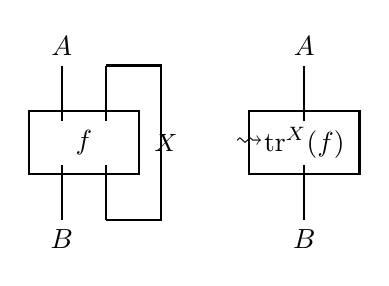
\begin{tikzpicture}[baseline=(current bounding box.center), scale=0.7]
  % Box f
  \node[draw, thick, minimum width=1.4cm, minimum height=0.8cm] (f) at (0,0) {$f$};
  % top inputs
  \draw[thick] (-0.4, 0.4) -- (-0.4, 1.4);
  \draw[thick] (0.4, 0.4) -- (0.4, 1.4);
  % bottom outputs
  \draw[thick] (-0.4, -0.4) -- (-0.4, -1.4);
  \draw[thick] (0.4, -0.4) -- (0.4, -1.4);
  % trace loop (X feedback)
  \draw[thick] (0.4, -1.4) -- (1.4, -1.4) -- (1.4, 1.4) -- (0.4, 1.4);
  % labels
  \node[above] at (-0.4, 1.4) {$A$};
  \node[below] at (-0.4, -1.4) {$B$};
  \node[right] at (1.1, 0)    {\small$X$};
  % equality + traced morphism
  \node at (3, 0) {$\;\rightsquigarrow\;$};
  \begin{scope}[xshift=4cm]
    \node[draw, thick, minimum width=1.4cm, minimum height=0.8cm]
      (trf) at (0,0) {$\mathrm{tr}^X(f)$};
    \draw[thick] (0, 0.4) -- (0, 1.4);
    \draw[thick] (0, -0.4) -- (0, -1.4);
    \node[above] at (0, 1.4) {$A$};
    \node[below] at (0, -1.4) {$B$};
  \end{scope}
\end{tikzpicture}
\end{center}
The four trace axioms~\cite{JSV} are:
\begin{itemize}
  \item \emph{Naturality} (left and right):
        $\mathrm{tr}^X(g \otimes \id_X \circ f) = g \circ \mathrm{tr}^X(f)$
        and analogously on the right.
  \item \emph{Dinaturality} (also called \emph{strength}):
        $\mathrm{tr}^X((\id_B \otimes h) \circ f) =
         \mathrm{tr}^Y(f \circ (\id_A \otimes h))$
        for $h : X \to Y$.
  \item \emph{Vanishing}:
        $\mathrm{tr}^I(f) = f$ (the unit object traces trivially) and
        $\mathrm{tr}^{X \otimes Y}(f) = \mathrm{tr}^X(\mathrm{tr}^Y(f))$
        (nested traces collapse).
  \item \emph{Superposing}:
        $\mathrm{tr}^X(\id_C \otimes f) = \id_C \otimes \mathrm{tr}^X(f)$.
  \item \emph{Yanking}: $\mathrm{tr}^X(\sigma_{X,X}) = \id_X$.
\end{itemize}

\paragraph{Intuition.}
The axioms say loops can be slid around (naturality), nested
(vanishing), moved past parallel boxes (superposing), and a wire
crossed and immediately re-routed to itself is a straight wire
(yanking).  This last axiom is the most visually striking:
\begin{center}
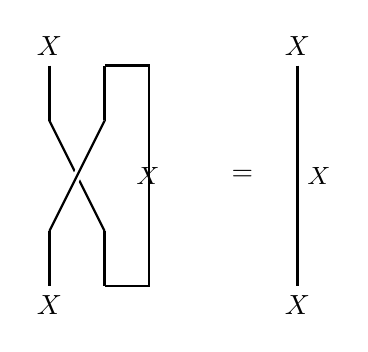
\begin{tikzpicture}[baseline=(current bounding box.center), scale=0.7]
  % LHS: braiding σ_{X,X} with right strand traced out
  \begin{scope}
    % Wire extensions above the cross
    \draw[thick] (0, 2) -- (0, 1);
    \draw[thick] (1, 2) -- (1, 1);
    % The crossing: one strand goes from (0,1) to (1,-1); the other
    % from (1,1) to (0,-1) drawn with a gap to suggest "over".
    \draw[thick] (0, 1) -- (1, -1);
    \draw[thick, white, line width=3pt] (1, 1) -- (0, -1);
    \draw[thick] (1, 1) -- (0, -1);
    % Wire extensions below the cross
    \draw[thick] (0, -1) -- (0, -2);
    \draw[thick] (1, -1) -- (1, -2);
    % Trace loop on the right strand
    \draw[thick] (1, -2) -- (1.8, -2) -- (1.8, 2) -- (1, 2);
    % labels
    \node[above] at (0, 2) {$X$};
    \node[below] at (0, -2) {$X$};
    \node[right] at (1.4, 0) {\small$X$};
  \end{scope}
  % Equality
  \node at (3.5, 0) {$=$};
  % RHS: straight X wire
  \begin{scope}[xshift=4.5cm]
    \draw[thick] (0, 2) -- (0, -2);
    \node[above] at (0, 2) {$X$};
    \node[below] at (0, -2) {$X$};
    \node[right] at (0, 0) {\small$X$};
  \end{scope}
\end{tikzpicture}
\end{center}
The trace loop and the braiding cancel out: following the strand,
it crosses, loops around, and crosses back to its starting column,
giving the identity.  This ``string diagram'' picture is rigorous:
\cite{JSV} (see also \cite{Selinger} for a survey) show that two
terms denote equal morphisms iff their string diagrams are isotopic
in the plane (with appropriate boundary conditions).

\paragraph{Examples.}
\begin{itemize}
  \item In any compact-closed category (e.g.\ finite-dimensional
        vector spaces with their tensor product, or finite sets with
        cartesian product but only including isomorphisms),
        $\mathrm{tr}^X(f) := (\rho_B \otimes \id) \circ (\id_B \otimes \mathrm{cap}_X)
        \circ (f \otimes \id_{X^*}) \circ (\id_A \otimes \mathrm{cup}_X) \circ (\rho_A^{-1})$.
  \item The category of partial recursive functions with cartesian
        product, where trace gives the minimisation/fixpoint operator.
  \item The Kleisli category of a monad equipped with an iteration
        operator (Hasegawa 1997) --- this is the setting for $\SFunM$
        with the coproduct tensor in Step 3.
\end{itemize}

\subsection{Compact closed categories}
\label{sec:compact}

A symmetric monoidal category $(\mathcal{C}, \otimes, I, \sigma)$ is
\emph{compact closed} if every object $A$ has a \emph{dual} $A^*$
equipped with two morphisms
\[
  \eta_A : I \to A \otimes A^*
  \qquad \text{(\emph{unit}, ``cup'')},
\]
\[
  \varepsilon_A : A^* \otimes A \to I
  \qquad \text{(\emph{counit}, ``cap'')},
\]
satisfying the \emph{snake} (also called \emph{zigzag} or
\emph{triangle}) identities
\begin{align*}
  (\id_A \otimes \varepsilon_A) \circ (\eta_A \otimes \id_A) &= \id_A,\\
  (\varepsilon_A \otimes \id_{A^*}) \circ (\id_{A^*} \otimes \eta_A) &= \id_{A^*}.
\end{align*}
In string-diagram notation $\eta_A$ is a U-shaped wire and
$\varepsilon_A$ is an upside-down U; the snake identities say a U
followed by an inverted U gives a straight wire:
\begin{center}
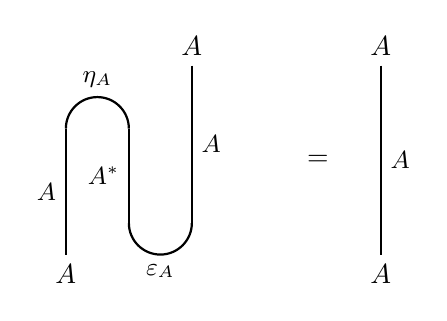
\begin{tikzpicture}[baseline=(current bounding box.center), scale=0.8]
  % LHS: zigzag through a cap (η) and cup (ε)
  \begin{scope}
    % Straight wire segments
    \draw[thick] (0,2) -- (0,0);                 % left output A
    \draw[thick] (1,2) -- (1,0.5);               % middle A^*
    \draw[thick] (2,3) -- (2,0.5);               % right input A
    % η: arc connecting (0,2) and (1,2), opening upward
    \draw[thick] (0,2) arc[start angle=180, end angle=0, radius=0.5];
    \node[above] at (0.5,2.5) {\small$\eta_A$};
    % ε: arc connecting (1,0.5) and (2,0.5), opening downward
    \draw[thick] (1,0.5) arc[start angle=180, end angle=360, radius=0.5];
    \node[below] at (1.5,0) {\small$\varepsilon_A$};
    % endpoint labels
    \node[above] at (2,3) {$A$};
    \node[below] at (0,0) {$A$};
    % strand labels
    \node[left]  at (0,1)    {\small$A$};
    \node[left]  at (1,1.25) {\small$A^*$};
    \node[right] at (2,1.75) {\small$A$};
  \end{scope}
  % Equality
  \node at (4,1.5) {$=$};
  % RHS: straight identity wire
  \begin{scope}[xshift=5cm]
    \draw[thick] (0,3) -- (0,0);
    \node[above] at (0,3) {$A$};
    \node[below] at (0,0) {$A$};
    \node[right] at (0,1.5) {\small$A$};
  \end{scope}
\end{tikzpicture}
\end{center}
The dual identity (for $A^*$) is the mirror image.

\paragraph{Key consequences.}
\begin{itemize}
  \item \emph{Hom-set isomorphism}:
        $\mathcal{C}(A \otimes B,\, C) \;\cong\; \mathcal{C}(A,\, B^* \otimes C)$.
        Arguments can be ``bent'' freely between input and output sides.
  \item \emph{Trace for free}: every compact-closed category is
        traced, with
        $\mathrm{tr}^X(f) :=
          (\id_B \otimes \varepsilon_X) \circ (f \otimes \id_{X^*}) \circ
          (\id_A \otimes \eta_X)$
        (modulo unitor isomorphisms).  Conversely, the G-construction
        below shows every traced category sits inside a compact-closed
        one as a sub-monoidal category.
  \item \emph{String diagrams} for a compact-closed category are
        isotopic in the plane up to deformation that takes strands
        through each other ``around'' a cup-cap pair --- strands can
        be bent freely, not just slid past each other.
\end{itemize}

\paragraph{Examples.}
\begin{itemize}
  \item $(\mathbf{FinVect}_k, \otimes_k, k)$ with $A^*$ the linear
        dual; $\eta$ is the canonical pairing $k \to A \otimes A^*$
        and $\varepsilon$ is evaluation $A^* \otimes A \to k$.
  \item $(\mathbf{Rel}, \times, 1)$ (sets and relations) with
        $A^* = A$ and $\eta, \varepsilon$ the diagonals.
  \item The G-construction $G\mathcal{C}$ of any traced symmetric
        monoidal $\mathcal{C}$, with $(A^+, A^-)^* := (A^-, A^+)$.
        Joyal--Street--Verity~\cite{JSV} prove that $G$ is in fact the
        free compact-closed category on $\mathcal{C}$ in an
        appropriate 2-categorical sense.
\end{itemize}

\subsection{The G-construction (``Int'' / Geometry of Interaction)}
\label{sec:gconstr}

Given a traced symmetric monoidal category $\mathcal{C}$, the
\emph{G-construction}~\cite{JSV} (sometimes called
the ``Int construction'' or ``Geometry of Interaction
construction'') produces a new category $G\mathcal{C}$ which is
\emph{compact closed}:
\begin{itemize}
  \item objects: pairs $(A^+, A^-) \in \Obj(\mathcal{C}) \times \Obj(\mathcal{C})$;
  \item morphisms $(A^+, A^-) \to (B^+, B^-)$:
        $\mathcal{C}\bigl(A^+ \otimes B^-,\; A^- \otimes B^+\bigr)$.
\end{itemize}
The intuition: $(A^+, A^-)$ is a wire with two directions ---
$A^+$ is the ``positive'' direction (information flowing forward),
$A^-$ is the ``negative'' direction (information flowing backward,
e.g.\ a request answered later).  A morphism shuffles incoming
flows ($A^+$ and $B^-$) into outgoing flows ($A^-$ and $B^+$).  This
is exactly the data of a \emph{bidirectional channel}.

\paragraph{Identity and composition.}
Identity at $(A^+, A^-)$ is the braiding
$\sigma : A^+ \otimes A^- \to A^- \otimes A^+$.  Composition of
$f : A^+ \otimes B^- \to A^- \otimes B^+$ with
$g : B^+ \otimes C^- \to B^- \otimes C^+$ is given by tracing out
the shared $B$:
\[
  g \circ_G f \;:=\; \mathrm{tr}^{B^+ \otimes B^-}\!\bigl(
                      \Phi \circ (f \otimes g) \circ \Psi
                    \bigr),
\]
where $\Phi$ and $\Psi$ are the symmetry-and-associator isomorphisms
that arrange the tensor factors so the shared $B$-component is
adjacent.  Intuitively: glue the $B$-output of $f$ to the $B$-input
of $g$ and trace the loop.

\begin{theorem}[\cite{JSV}]
$G\mathcal{C}$ is a compact-closed category.  The assignment
$A \mapsto (A, I)$ extends to a strong monoidal functor
$\mathcal{C} \to G\mathcal{C}$ which is fully faithful onto a
sub-monoidal-category of objects of the form $(A, I)$.
\end{theorem}

\paragraph{Compact closure.}
Being compact closed (see Appendix~\ref{sec:compact}) means every
object $(A^+, A^-)$ has a \emph{dual}, $(A^+, A^-)^* = (A^-, A^+)$,
with unit and counit morphisms (``cup'' and ``cap''):
\[
  \eta : I \to (A^+, A^-) \otimes (A^+, A^-)^*,
  \qquad
  \epsilon : (A^+, A^-)^* \otimes (A^+, A^-) \to I.
\]
This is exactly the structure needed to interpret feedback,
recursion, and the channel-transpose $(-)^T$ of
\texttt{Channel.Core}.

\paragraph{Why it's the right structure for channels.}
A typed channel $A$ in this development has \emph{in-type} and
\emph{out-type}; the pair $(A^+, A^-)$ in $G\SFunM$ matches the
in/out data of a channel.  A morphism from channel $A$ to channel $B$
in $G\SFunM$ is a stateful monadic function
$A^+ \sqcup B^- \to A^- \sqcup B^+$ --- i.e.\ ``given an input on
$A$'s in-side or $B$'s out-side, emit on $A$'s out-side or $B$'s
in-side''.  That is precisely a bidirectional step function on the
combined channel $A \otimes B^T$.  The G-construction therefore
\emph{re-creates the type discipline of typed channels} from the
underlying category of stateful processes.



\begin{thebibliography}{Hasegawa97}

\bibitem[Bec67]{Beck}
  Jonathan~Beck. 1967.
  \newblock \emph{Triples, algebras and cohomology}.
  \newblock Ph.D.\ thesis, Columbia University.  Republished in
  \emph{Reprints in Theory and Applications of Categories} (2003).

\bibitem[BÉ93]{BloomEsik}
  Stephen L.\ Bloom and Zolt\'an \'Esik. 1993.
  \newblock \emph{Iteration Theories: The Equational Logic of
                  Iterative Processes}.
  \newblock EATCS Monographs on Theoretical Computer Science,
                  Springer.

\bibitem[Has97]{Hasegawa97}
  Masahito Hasegawa. 1997.
  \newblock Recursion from cyclic sharing: Traced monoidal
            categories and models of cyclic lambda-calculi.
  \newblock In \emph{Typed Lambda Calculi and Applications (TLCA)},
            LNCS 1210, pp.~196--213.

\bibitem[JSV96]{JSV}
  Andr\'e Joyal, Ross Street, and Dominic Verity. 1996.
  \newblock Traced monoidal categories.
  \newblock \emph{Mathematical Proceedings of the Cambridge
                  Philosophical Society} 119(3): 447--468.

\bibitem[Kat14]{Katsumata}
  Shin-ya Katsumata. 2014.
  \newblock Parametric effect monads and semantics of effect
            systems.
  \newblock In \emph{Principles of Programming Languages (POPL)},
            ACM, pp.~633--645.

\bibitem[ML63]{MacLane63}
  Saunders Mac Lane. 1963.
  \newblock Natural associativity and commutativity.
  \newblock \emph{Rice University Studies} 49(4): 28--46.

\bibitem[ML98]{CWM}
  Saunders Mac Lane. 1998.
  \newblock \emph{Categories for the Working Mathematician},
            2nd~edition.
  \newblock Graduate Texts in Mathematics 5, Springer.

\bibitem[Man76]{Manes}
  Ernest~G.\ Manes. 1976.
  \newblock \emph{Algebraic Theories}.
  \newblock Graduate Texts in Mathematics 26, Springer.

\bibitem[Mog91]{Moggi}
  Eugenio Moggi. 1991.
  \newblock Notions of computation and monads.
  \newblock \emph{Information and Computation} 93(1): 55--92.

\bibitem[PP02]{PlotkinPower}
  Gordon Plotkin and John Power. 2002.
  \newblock Notions of computation determine monads.
  \newblock In \emph{Foundations of Software Science and Computation
                     Structures (FoSSaCS)}, LNCS 2303, pp.~342--356.

\bibitem[Sel11]{Selinger}
  Peter Selinger. 2011.
  \newblock A survey of graphical languages for monoidal
            categories.
  \newblock In B.~Coecke (ed.), \emph{New Structures for Physics},
            Lecture Notes in Physics 813, Springer,
            pp.~289--355.

\end{thebibliography}

\end{document}
